\chapter*{CI-2-3 track}
\addcontentsline{toc}{chapter}{CI-2-3 track}
\label{ci-track}

\begin{figure}[h!]
\centering
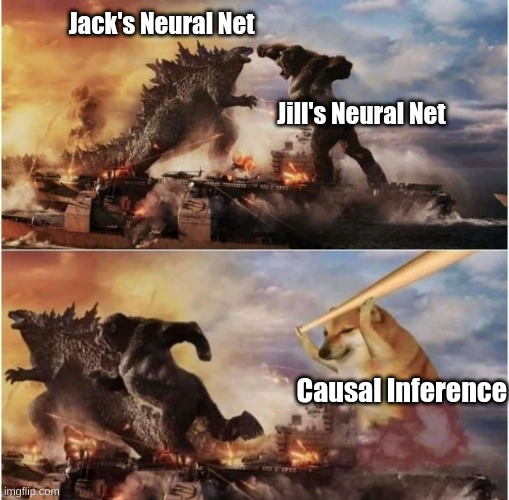
\includegraphics[width=5in]
{godzilla-kk-doge-nn-ci.jpg}
\caption{CI meme} 
\label{fig-godzilla-kk-doge}
\end{figure}

As discussed in Chapter \ref{ch-counterf},
Judea Pearl has proposed 3 rungs 
of Causal Inference (CI).
This book covers all 3 rungs.
Some people (for instance,
economists)\footnote{This is evinced by
the excellent books Refs.\cite{book-mixtape},
and \cite{alves-book}
written by economists.}
are mostly interested in the highest
2 rungs; i.e, 
rung 2 (do operations)
and rung 3 (imagining/counterfactual thinking).
Here is a subset of chapters
that I call
the CI-2-3 track,
that are devoted mostly to rungs 2 and 3. 


\begin{enumerate}
\item \nameref{ch-bdoor}
\item \nameref{ch-counterf}
\item \nameref{ch-did}
\item \nameref{ch-do-calc}
\item \nameref{ch-dsep}
\item \nameref{ch-fwl-theo}
\item \nameref{ch-fdoor}
\item \nameref{ch-good-causal-fit}
\item \nameref{ch-granger-c}
\item \nameref{ch-inst-ineq}
\item \nameref{ch-instrumental}
\item \nameref{ch-meta-learners}
\item \nameref{ch-pot-out}
\item \nameref{ch-reg-dis}
\item \nameref{ch-syn-con}
\item \nameref{ch-uplift}
\end{enumerate}